\section{VAM Vorticity Scattering Framework (inspired by elastic theory)}

\subsection{Governing equations of VAM Vorticity dynamics}

\subsubsection*{Vorticity transport equation (linearized form)}

In the Vortex Æther Model (VAM), the dynamics of the vorticity field \(\vec{\omega} = \nabla \times \vec{v}\) is governed by the Euler equation and the associated vorticity form:

\[
    \frac{\partial \omega_i}{\partial t} + v_j \partial_j \omega_i = \omega_j \partial_j v_i
\]

This nonlinear structure implies vortex deformation by stretching and advection. For small perturbations \(\delta\omega\) near a background vortex node field \(\omega^{(0)}\) linearization yields:

\[
    \frac{\partial (\delta \omega_i)}{\partial t} + v_j^{(0)} \partial_j (\delta \omega_i) \approx \omega_j^{(0)} \partial_j (\delta v_i)
\]

Define the linear response operator of VAM \(\mathcal{L}_{ij}\):

\[
    \mathcal{L}_{ij} \, \delta v_j(\vec{r}) = \delta F_i^\text{vortex}(\vec{r})
\]

\subsubsection*{Green Tensor Vorticity Equation}

\[
    \mathcal{L}_{ij} \, \mathcal{G}_{jk}(\vec{r}, \vec{r}') = -\delta_{ik} \, \delta(\vec{r} - \vec{r}')
\]

The induced velocity field \(v_i\) of a source vortex force \(F_k(\vec{r}')\) is then:

\[
    v_i(\vec{r}) = \int \mathcal{G}_{ik}(\vec{r}, \vec{r}') \, F_k^\text{vortex}(\vec{r}') \, d^3 r'
\]

\subsection{Vortex filament interaction}
Interactions arise from exchange of vortex force or Reconnections between vortex filaments:
\begin{itemize}
    \item Attractive when filaments reinforce the circulation (parallel)
    \item Repulsive when filaments cancel each other out (antiparallel)
    \item Interaction strength:
\end{itemize}
\begin{equation}
    \vec{F}_\text{int} = \beta \cdot \kappa_1 \kappa_2 \cdot \frac{\vec{r}_{12} \times (\vec{v}_1 - \vec{v}_2)}{|\vec{r}_{12}|^3}\label{eq:interaction_strength}
\end{equation}
Where \(\kappa_i\) are the circulations of filaments and \(\vec{r}_{12}\) is the vector between them.

\subsection{Thermodynamic \& quantum behavior of vorticity fluctuations}
\begin{itemize}
    \item Entropy \(\leftrightarrow\) volume of vortex expansion or knot deformation
    \item Quantum transitions \(\leftrightarrow\) topological reconnection events
    \item Zero-point motion \(\leftrightarrow\) background quantum turbulence of the Æther:
\end{itemize}

\subsubsection*{Quantum vorticity background}
\begin{equation}
    \langle \omega^2 \rangle \sim \frac{\hbar}{\rho_\text{æ} \xi^4}\label{eq:quantum_vorticity_background}
\end{equation}
Where \(\xi\) is the coherence length between vortex filaments.

\subsection{VAM scattering theory for vortex nodes}

\subsubsection*{Born approximation for vortex perturbations}

Suppose that an incident vortex potential \(\Phi^{(0)}(\vec{r})\) encounters a vortex node at \(\vec{r}_k\). The scattered vorticity field becomes:

\[
    \Phi(\vec{r}) = \Phi^{(0)}(\vec{r}) + \int \mathcal{G}_{ij}(\vec{r}, \vec{r}') \, \delta \mathcal{V}_{jk}(\vec{r}') \, v_k^{(0)}(\vec{r}') \, d^3r'
\]

Here \(\delta \mathcal{V}_{jk}\) represents a vorticity polarization tensor associated with the node – a VAM analogue of elastic moduli perturbation.

\subsection{Æther stress tensor and energy flux}

\subsubsection*{VAM stress tensor}

\[
    \mathcal{T}_{ij} = \rho_\text{\ae} \, v_i v_j - \frac{1}{2} \delta_{ij} \rho_\text{\ae} v^2
\]

\subsubsection*{Æther Vorticity Force Density}

\[
    f_i^\text{vortex} = \partial_j \mathcal{T}_{ij}
\]

\subsubsection*{Vorticity Energy Flux}

\[
    \vec{S}_\omega = - \mathcal{T} \cdot \vec{v}
\]

This vector captures the energy transfer via vortex node interactions and defines Scattering of "cross sections" via the divergence \(\nabla \cdot \vec{S}_\omega\).

\subsection{Time dilation and nodal scattering}

\subsubsection*{Chronos-Time Delay due to Nodal Rotation}

\[
    \frac{d\tau}{d\mathcal{N}} = \left(1 + \frac{1}{2} \beta I \Omega_k^2 \right)^{-1}
\]

Here, \( \tau \) is the local Chronos-Time (observer-proper time), and $\mathcal{N}$ is the global Aithēr-Time. This relation defines how temporal flow is modulated at vortex scattering sites due to stored rotational energy.


In the Born approximation, the change in proper time near a node under external vortex flow is:
\paragraph{Kairos Threshold} A sudden vortex reconnection or discontinuity in the background flow may generate a \emph{Kairos Moment} \( \kappa \), where irreversible topological rearrangement occurs.

\subsubsection*{Scattered correction due to external field}
All scattering processes are evaluated along the causal background frame defined by Aithēr-Time \( \mathcal{N} \), with local response times governed by \( \tau \) and swirl synchronization effects encoded in \( S(t) \).

\begin{gather*}
    \delta \left( \frac{d\tau}{d\mathcal{N}} \right)\approx - \frac{1}{2} \beta I \Omega_k \, \delta \Omega_k\\
    \delta \Omega_k \sim \int \chi(\vec{r}_k - \vec{r}') \cdot \vec{\omega}^{(0)}(\vec{r}') \, d^3r'\\
\end{gather*}

\subsubsection*{Swirl Clock Phase Shift}
\[
    \delta S(t) = \int_{t_0}^{t} \delta \omega_k(t') \, dt'
\]

$S(t)$ is the Swirl Clock variable — its phase is shifted during scattering due to perturbations in local vorticity. This contributes to temporal decoherence and phase drift.



Here \(\chi\) is the topological eddy sensitivity core.
\subsection{Summary of VAM-inspired scattering structures}

\begin{table}[htbp]
    \centering
    \begin{tabular}{lll}
        \toprule
    \textbf{Concept} & \textbf{Elastic theory} & \textbf{VAM analogue} \\
    \midrule
    Medium property & \( c_{ijkl} \) & \( \rho_\text{\ae},\, \Omega_k,\, \kappa \) \\
    Wavefield & \( u_i \) (displacement) & \( v_i \) (æther velocity) \\
    Source & \( f_i \) (body force) & \( F_i^\text{vortex} \) (vorticity forcing) \\
    Green function & \( G_{ij}(\vec{r}, \vec{r}') \) & \( \mathcal{G}_{ij}(\vec{r}, \vec{r}') \) \\
    Stress tensor & \( \tau_{ij} \) & \( \mathcal{T}_{ij} \) \\
    Energy flux & \( J_{P,i} = -\tau_{ij} \dot{u}_j \) & \( S_{\omega,i} = -\mathcal{T}_{ij} v_j \) \\
    Time dilation mechanism & \( g_{\mu\nu} \) (GR metric) & \( \Omega_k,\, \kappa,\, \langle \omega^2 \rangle \) \\
    \bottomrule
    \end{tabular}
    \caption{Conceptual correspondence between classical elasticity and Vortex Æther Model (VAM).}
    \label{tab:elastic-vam-analogy}
\end{table}

This scattering framework generalizes classical elastic analogs to a topologically and energetically motivated Ætheric formalism. It allows the calculation of field modifications, time dilation effects, and energy flux due to stable, interacting vortices in the Vortex Æther Model (VAM).

\begin{figure}[H]
\centering
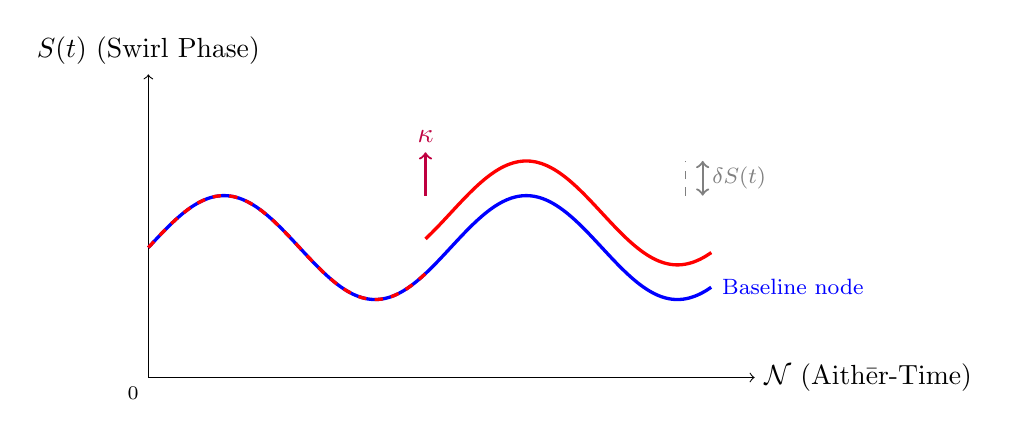
\begin{tikzpicture}[scale=1.1]

% Axes
\draw[->] (0,0) -- (7,0) node[right] {\( \mathcal{N} \) (Aithēr-Time)};
\draw[->] (0,0) -- (0,3.5) node[above] {\( S(t) \) (Swirl Phase)};

% Baseline trajectory
\draw[very thick, blue] plot[smooth,domain=0:6.5,samples=100]
    (\x, {1.5 + 0.6*sin(1.8*\x r)}) node[right] {\footnotesize Baseline node};

% Shifted trajectory (after Kairos Moment)
\draw[very thick, red, dashed]
    plot[domain=0:3.2,samples=50,smooth]
    (\x, {1.5 + 0.6*sin(1.8*\x r)});

\draw[very thick, red]
    plot[domain=3.2:6.5,samples=50,smooth]
    (\x, {1.9 + 0.6*sin(1.8*\x r)});
    node[right] {\footnotesize Scattered node};

% Kairos Moment arrow
\draw[->, thick, purple] (3.2,2.1) -- (3.2,2.6);
\node[above, purple] at (3.2,2.6) {\( \kappa \)};

% Phase shift annotation
\draw[dashed, gray] (6.2,2.1) -- (6.2,2.5);
\draw[<->, thick, gray] (6.4,2.1) -- (6.4,2.5);
\node[right, gray] at (6.4,2.3) {\footnotesize \( \delta S(t) \)};

% Labels
\node[below left] at (0,0) {\scriptsize 0};

\end{tikzpicture}
\caption{Swirl Clock phase shift due to a transient vorticity wave in VAM.
The baseline node (blue) maintains a steady Swirl Clock evolution.
The scattered node (red) experiences a permanent phase offset \( \delta S(t) \) after a transient rotation perturbation, marking a \emph{Kairos Moment} \( \kappa \).}
\label{fig:swirl_phase_shift}
\end{figure}

\begin{itemize}
\item X-axis: Aithēr-Time $\mathcal{N}$, the global causal time.
\item Y-axis: Swirl Clock phase $S(t)$, encoding rotational state.
\item Blue curve: A vortex node unaffected by external waves.
\item Red curve: A node perturbed by a vorticity wave — its phase shifts permanently after $\kappa$.
\item Arrow $\kappa$: Marks the \textit{irreversible bifurcation}, representing a real physical transition, not just coordinate transformation.
\end{itemize}




\begin{figure}[H]
\centering
\begin{tikzpicture}[scale=1.05]

% Axes
\draw[->] (0,0) -- (7,0) node[right] {\( \mathcal{N} \) (Aithēr-Time)};
\draw[->] (0,0) -- (0,3.2) node[above] {\( S(t) \) (Swirl Phase)};

% Node A: unaffected
\draw[very thick, blue] plot[smooth,domain=0:6.5,samples=100]
    (\x, {1.0 + 0.5*sin(2*\x r)}) node[right] {\footnotesize Node A (Reference)};

% Node B: affected by wave
\draw[very thick, red, dashed]
    plot[smooth,domain=0:3,samples=100]
    (\x, {2.0 + 0.5*sin(2*\x r)});

\draw[very thick, red]
    plot[smooth,domain=3:6.5,samples=100]
    (\x, {2.3 + 0.5*sin(2*\x r)}) node[right] {\footnotesize Node B (Perturbed)};

% Kairos Moment
\draw[->, thick, purple] (3,2.5) -- (3,3.0);
\node[above, purple] at (3,3.0) {\( \kappa \)};

% Phase shift
\draw[<->, thick, gray] (6.4,{1.0+0.5*sin(deg(13))}) -- (6.4,{2.3+0.5*sin(deg(13))});
\node[right, gray] at (6.4,1.7) {\footnotesize \( \delta S(t) \)};

% Dotted line connecting nodes before wave
\draw[dashed, teal] (0,1.0) -- (0,2.0);
\node[left, teal] at (0,1.5) {\scriptsize Synchronized};

% Dotted line connecting nodes after wave
\draw[dashed, teal] (6.5,1.0+0.5*sin(deg(13)* r)) -- (6.5,2.3+0.5*sin(deg(13)* r));
\node[left, teal] at (6.5,2.1) {\scriptsize Desynchronized};

% Origin label
\node[below left] at (0,0) {\scriptsize 0};

\end{tikzpicture}
\caption{
\textbf{Ætheric Gravitational Wave as Swirl Clock Phase Drift.}
A transient vorticity perturbation shifts the Swirl Clock \( S(t) \) of Node B relative to Node A.
The shift occurs at a Kairos Moment \( \kappa \), producing a lasting phase lag \( \delta S(t) \).
This phase decoherence represents a VAM analog to gravitational waves, where time differences arise from topological swirl transitions rather than spacetime curvature.
}
\label{fig:swirl_clock_wavefront}

\end{figure}

\begin{itemize}
\item Causal Time $\mathcal{N}$ runs along the x-axis — it's global and universal.
\item Both nodes start synchronized: $S_A(t) = S_B(t)$
\item After the wave passes Node B at time $\mathcal{N}_\kappaN$, its swirl phase shifts: $\delta S(t) \ne 0$
\item This phase difference is \textit{observable} and \textit{permanent}, just like the distance shift in GR interferometers — but here it's swirl clock drift.
\end{itemize}



\subsubsection*{Temporal Ontology Integration in Scattering}

\begin{itemize}
    \item \textbf{Aithēr-Time} \( \mathcal{N} \): Governs causal background evolution; all scattering propagators \( \mathcal{G}_{ij} \) evolve over \( d\mathcal{N} \).
    \item \textbf{Chronos-Time} \( \tau \): Locally dilated at each node depending on angular inertia \( I \Omega_k^2 \).
    \item \textbf{Swirl Clock} \( S(t) \): Phase-shifted due to incoming vorticity \( \vec{\omega}^{(0)} \), measurable via beat frequencies in scattered flow.
    \item \textbf{Kairos Moment} \( \kappa \): Triggered when \(\delta \Omega_k \gg \Omega_k\), marking a topological bifurcation.
\end{itemize}

\subsubsection*{External Observer Frame}

In experimental setups, vortex scattering effects are measured in laboratory time \( \bar{t} \), distinct from local vortex proper time \( \tau \). Their ratio approximates:

\[
    \frac{d\tau}{d\bar{t}} = \frac{\omega_\text{obs}}{\omega_k} \quad \text{(Chronos vs. External Clock rate via observed vs intrinsic swirl)}

\]

Where \( \omega_\text{obs} \) is the observed vortex beat frequency and \( \omega_k \) is the swirl eigenfrequency of the node.
